\documentclass[fleqn,portrait]{betterposter}

% Draw some nice diagrams
\usepackage{tikz}
\usetikzlibrary{backgrounds}
\usetikzlibrary{arrows}
\tikzstyle{directed-top}=[->, very thick, white, line width=0.1em, tikzit draw=black]
\pgfkeys{/tikz/tikzit draw/.initial=0}
\pgfdeclarelayer{edgelayer}
\pgfdeclarelayer{nodelayer}
\pgfsetlayers{backgroundlayer,main,notelayer,edgelayer,nodelayer}
\tikzstyle{none}=[inner sep=0mm]
%

\begin{document}

% Upper row
\betterThreeColumns{
  \title{The Title}
  \vspace{-1em}
  \author{Mike Morrison and Rafael Bailo}
  \institution{Optional Institution Under Name}

  \section{Introduction}
  Here is an itemised list:
  \begin{itemize}
    \item The first item.
    \item The second item.
    \item The third item.
  \end{itemize}
}{
  \section{A Diagram}
  Here is a diagram:
  \begin{center}
    % Linear regression
    % Author: Henri Menke
    % Retrieved from: http://www.texample.net/tikz/examples/linear-regression/
    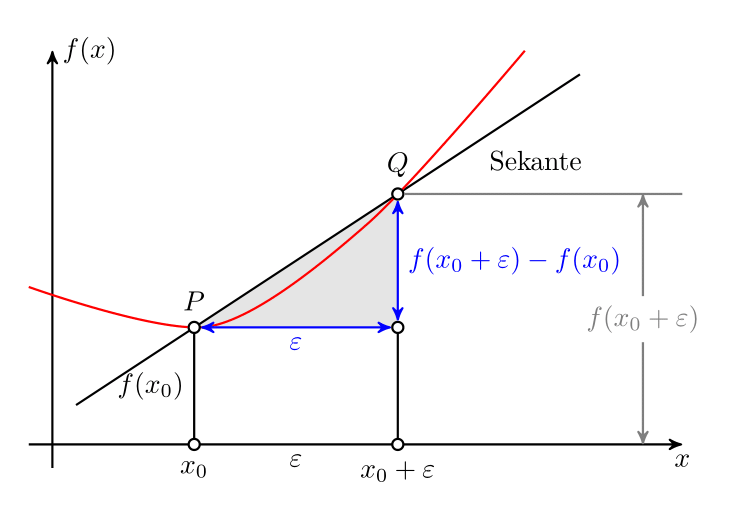
\includegraphics[width=.3\textwidth]{img/tikzexample1}
  \end{center}
}{
  \section{Fundamental Theorem\\of Calculus}
  If \(f\) is continuous on the closed interval \([a,b]\) and \(F\) is the indefinite integral of \(f\) on \([a,b]\), then
  \begin{equation}
    \int_a^b f(x)\,\mathrm{d}x = F(b)-F(a).
  \end{equation}

  \section{Conclusion}
  This is a great poster format!
}

% Middle row
\maincolumn{\centering
  \bigskip\bigskip\bigskip\bigskip\bigskip\bigskip

  \textbf{Main finding} goes here,\\[-1em]
  translated into \textbf{plain English}.\\[-1em]
  \textbf{Emphasize} the important words.

  \vfill

  %% QR code
  \begin{minipage}[t][][b]{0.90\textwidth}
    \begin{minipage}{0.13\textwidth}
      \qrcode[nolinks, height=10cm]{https://arxiv.org/abs/2301.03545}
    \end{minipage}%
    \fontsizestandard
    \begin{minipage}[t][0.07\textheight][b]{0.24\textwidth}
      \begin{tikzpicture}[scale=3]
        \begin{pgfonlayer}{nodelayer}
          \node [style=none] (0) at (2, 0.5) {};
          \node [style=none] (1) at (0.5, 2) {};
          \node [style=none] (2) at (2, 0) {Get the paper here!};
        \end{pgfonlayer}
        \begin{pgfonlayer}{edgelayer}
          \draw [style=directed-top, in=0, out=90] (0.center) to (1.center);
        \end{pgfonlayer}
      \end{tikzpicture}
    \end{minipage}%
  \end{minipage}

 \bigskip\bigskip\bigskip\bigskip\bigskip\bigskip
}

% Bottom row
\betterThreeColumns{
  Here you can add \textbf{supplementary material}. For instance, a new diagram:
  \begin{center}
    % Commutative diagram with edges passing under/over
    % Author: Stefan Kottwitz, http://texblog.net/
    % Retrieved from: http://www.texample.net/tikz/examples/commutative-diagram/
    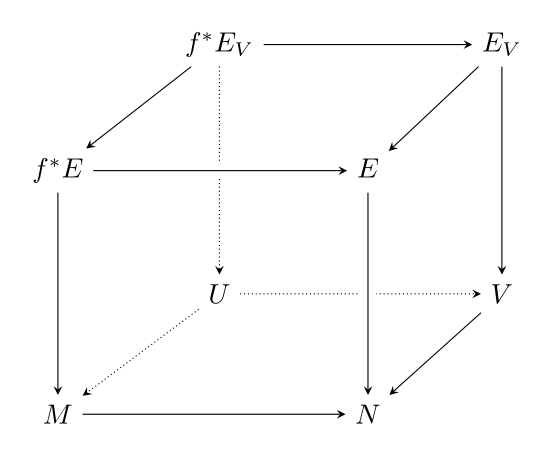
\includegraphics[width=.3\textwidth]{img/tikzexample2}
  \end{center}
}{
  Some cute ducklings:
  \begin{center}
    % Picture of ducklings
    % Author: Magda Ehlers, https://www.pexels.com/@magda-ehlers-pexels
    % Retrieved from: https://www.pexels.com/photo/selective-focus-photo-of-flock-of-ducklings-perching-on-gray-concrete-pavement-1300355/
    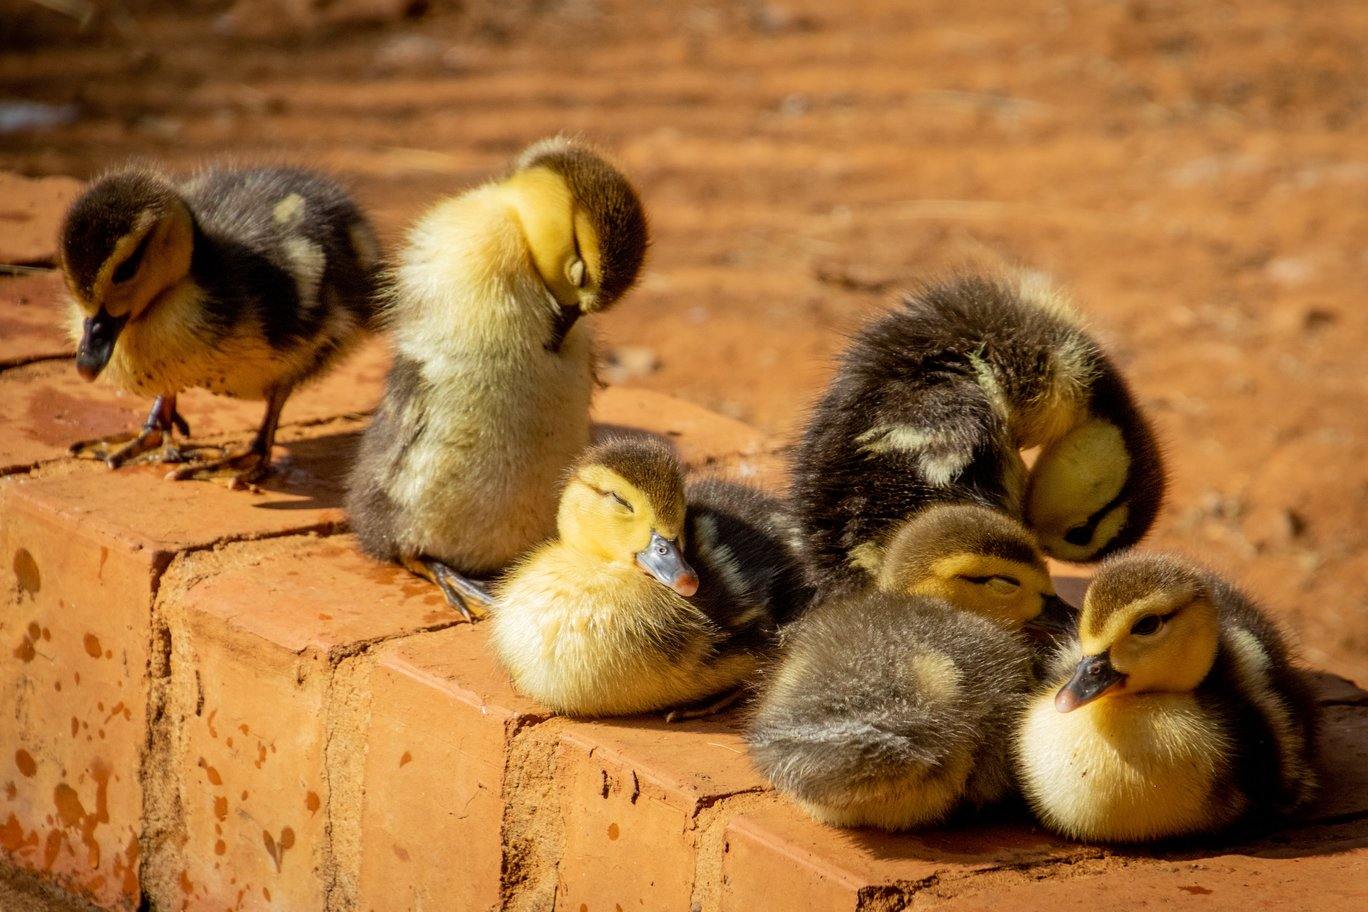
\includegraphics[width=.3\textwidth]{img/ducklings}
  \end{center}
}{
  And so on.
}

\end{document}
